\documentclass[a4paper, 18pt]{article}
\usepackage[T1]{fontenc}
\usepackage[portuguese]{babel}
\usepackage[utf8]{inputenc}
\usepackage[margin=3cm,includefoot,footskip=30pt,]{geometry}

\usepackage{graphicx}
\graphicspath{ {imagens/} }
\usepackage{bold-extra}
\usepackage{epstopdf}
\usepackage{float}
\usepackage{scalerel}
\usepackage{enumerate}
\usepackage{indentfirst}
\usepackage{mathtools}
\usepackage{amsmath}
\allowdisplaybreaks
\usepackage{cleveref}
\usepackage{amssymb}
\usepackage{listings}
\usepackage{color}
\newcommand\showdiv[1]{\overline{\smash{\hstretch{.5}{)}\mkern-3.2mu\hstretch{.5}{)}}#1}}
\newcommand\ph[1]{\textcolor{white}{#1}}


\definecolor{dkgreen}{rgb}{0,0.6,0}
\definecolor{gray}{rgb}{0.5,0.5,0.5}
\definecolor{mauve}{rgb}{0.58,0,0.82}
\definecolor{mygreen}{RGB}{28,172,0} % color values Red, Green, Blue
\definecolor{mylilas}{RGB}{170,55,241}

%\lstset{language=Matlab,%
%    %basicstyle=\color{red},
%    breaklines=true,%
%    morekeywords={matlab2tikz},
%    keywordstyle=\color{blue},
%    morekeywords=[2]{1}, keywordstyle=[2]{\color{black}},
%    identifierstyle=\color{black},
%    stringstyle=\color{mylilas},
%    commentstyle=\color{mygreen},
%    showstringspaces=false,
%	%inputencoding=utf8,
%	extendedchars=true,
%	literate={á}{{\'a}}1 {ã}{{\~a}}1 {â}{\^{a}}1 {é}{\'{e}}1 {ç}{\c{c}}1 {ã}{\~{a}}1 {à}{\`{a}}1 {ê}{\^{e}}1 {í}{\'{i}}1 {ó}{\'{o}}1 {õ}{\~{o}}1 {ô}{\^{o}}1 {ú}{\'{u}}1 {Ç}{\c{C}}1,
%}


\lstset{frame=tb,
  language=Matlab,
  aboveskip=3mm,
  belowskip=3mm,
  showstringspaces=false,
  columns=flexible,
  basicstyle={\small\ttfamily},
  numbers=none,
  numberstyle=\tiny\color{gray},
  keywordstyle=\color{blue},
  commentstyle=\color{dkgreen},
  stringstyle=\color{mauve},
  breaklines=true,
  breakatwhitespace=true,
  tabsize=3,
  extendedchars=true,
  literate=	{á}{{\'a}}1	{ã}{{\~a}}1	{â}{\^{a}}1	{é}{\'{e}}1	{ç}{\c{c}}1
  			{ã}{\~{a}}1	{à}{\`{a}}1 {ê}{\^{e}}1 {í}{\'{i}}1	{ó}{\'{o}}1
  			{õ}{\~{o}}1 {ô}{\^{o}}1	{ú}{\'{u}}1 {Ç}{\c{C}}1,
}

% ----- Cabeçalho e rodapé -----
\usepackage{fancyhdr}
\pagestyle{fancy}
\fancyhf{}

\renewcommand{\headrulewidth}{1pt}
\renewcommand{\footrulewidth}{0.5pt}

\rhead{Word Morph}
\lhead{Algoritmos e Estruturas de Dados\rightmark}
\rfoot{Página \thepage}
\lfoot{\small Engenharia Eletrotécnica e de Computadores - IST}


\usepackage{pdfpages}

\begin{document}
%Os relatórios devem ser entregues na altura indicada na Tabela 1. O relatório do pro-
%jecto deverá contemplar os aspectos seguidamente indicados. A apresentação do mesmo
%deverá iniciar-se por aspectos de ordem geral, seguindo-se descrições mais detalhadas dos
%módulos e estruturas de dados utilizados. Sugere-se a seguinte estrutura para o relatório:
%• Uma capa com os dados dos membros do grupo, incluindo nome, número e e-mail.
%Esta capa deverá seguir o formato indicado na página da disciplina (oportunamente
%será disponibilizado);
%• Uma página com o ı́ndice das secções em que o relatório se divide;
%• Uma descrição do problema que foi resolvido, com indicação clara das especificações
%do mesmo tal como foram entendidas;
%• Um texto simples que indique como os alunos abordaram e resolveram o problema;
%• Uma descrição completa da arquitectura do programa, incluindo fluxogramas de-
%talhados e um texto claro, mas sucinto, indicando a divisão lógica e funcional dos
%módulos desenvolvidos para a resolução do problema, explicitando os respectivos
%objectivos, as funções utilizadas e as estruturas de dados de suporte;
%• Uma descrição detalhada dos tipos de dados utilizadas e justificação dos mesmos
%(tabelas, listas, filas, pilhas, árvores, grafos, acervos, etc.);
%• Descrição dos algoritmos usados (por exemplo, na manipulação dos tipos de dados);
%• Uma descrição dos subsistemas funcionais que existam e, para cada um
%– a descrição dos objectivos do subsistema (até 5 linhas);
%– o nome do módulo onde estão definidos os tipos de dados abstractos (ficheiros
%.h) a utilizar no subsistema;
%– o nome do módulo C onde estão as funções do respectivo subsistema;
%– listagem das funções implementadas no subsistema, indicando para cada uma a
%respectiva assinatura e os objectivos da função (descrição sumária, sem código);
%• Uma análise, formal e/ou empı́rica, dos requisitos computacionais do programa
%desenvolvido, tanto em termos da memória que utiliza como da complexidade com-
%putacional, com particular ênfase no custo das operações de processamento sobre
%os tipos de dados usados e/ou criados;
%• Uma análise crı́tica do funcionamento do programa e a avaliação do desempenho
%do projecto implementado;
%• Pelo menos, um pequeno exemplo completo e detalhado de aplicação, com descrição
%da utilização das estruturas de dados em cada passo e de como são tomadas as
%decisões.

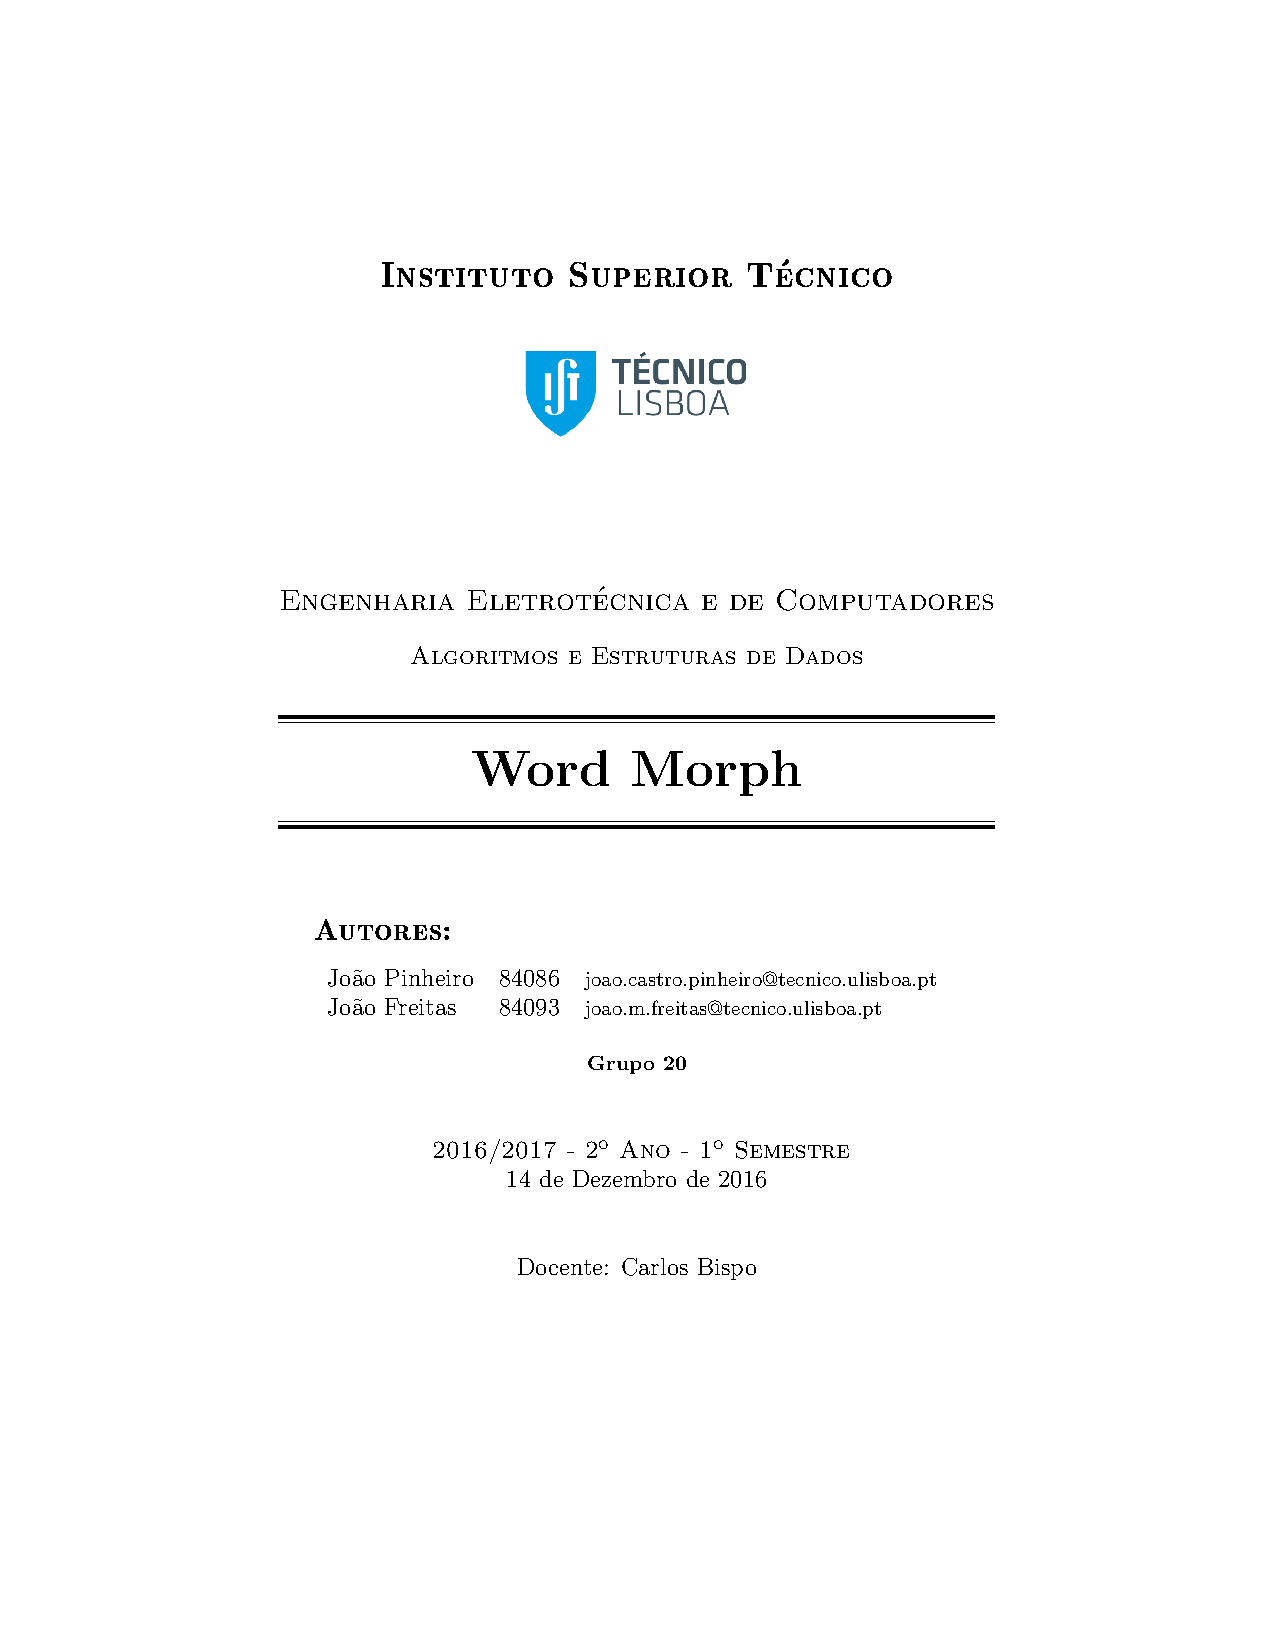
\includepdf[pages={1}]{capa/capa.pdf}

\end{document}
